\documentclass[]{article}
\usepackage{lmodern}
\usepackage{amssymb,amsmath}
\usepackage{ifxetex,ifluatex}
\usepackage{fixltx2e} % provides \textsubscript
\ifnum 0\ifxetex 1\fi\ifluatex 1\fi=0 % if pdftex
  \usepackage[T1]{fontenc}
  \usepackage[utf8]{inputenc}
\else % if luatex or xelatex
  \ifxetex
    \usepackage{mathspec}
  \else
    \usepackage{fontspec}
  \fi
  \defaultfontfeatures{Ligatures=TeX,Scale=MatchLowercase}
\fi
% use upquote if available, for straight quotes in verbatim environments
\IfFileExists{upquote.sty}{\usepackage{upquote}}{}
% use microtype if available
\IfFileExists{microtype.sty}{%
\usepackage{microtype}
\UseMicrotypeSet[protrusion]{basicmath} % disable protrusion for tt fonts
}{}
\usepackage[margin=1in]{geometry}
\usepackage{hyperref}
\hypersetup{unicode=true,
            pdftitle={Framework to Estimate Snake Basin Steelhead and Chinook Population Abundance and Productivity},
            pdfauthor={Ryan N. Kinzer and Rick Orme; Chris Beasley, Kevin See and Mike Ackerman},
            pdfborder={0 0 0},
            breaklinks=true}
\urlstyle{same}  % don't use monospace font for urls
\usepackage{graphicx,grffile}
\makeatletter
\def\maxwidth{\ifdim\Gin@nat@width>\linewidth\linewidth\else\Gin@nat@width\fi}
\def\maxheight{\ifdim\Gin@nat@height>\textheight\textheight\else\Gin@nat@height\fi}
\makeatother
% Scale images if necessary, so that they will not overflow the page
% margins by default, and it is still possible to overwrite the defaults
% using explicit options in \includegraphics[width, height, ...]{}
\setkeys{Gin}{width=\maxwidth,height=\maxheight,keepaspectratio}
\IfFileExists{parskip.sty}{%
\usepackage{parskip}
}{% else
\setlength{\parindent}{0pt}
\setlength{\parskip}{6pt plus 2pt minus 1pt}
}
\setlength{\emergencystretch}{3em}  % prevent overfull lines
\providecommand{\tightlist}{%
  \setlength{\itemsep}{0pt}\setlength{\parskip}{0pt}}
\setcounter{secnumdepth}{0}
% Redefines (sub)paragraphs to behave more like sections
\ifx\paragraph\undefined\else
\let\oldparagraph\paragraph
\renewcommand{\paragraph}[1]{\oldparagraph{#1}\mbox{}}
\fi
\ifx\subparagraph\undefined\else
\let\oldsubparagraph\subparagraph
\renewcommand{\subparagraph}[1]{\oldsubparagraph{#1}\mbox{}}
\fi

%%% Use protect on footnotes to avoid problems with footnotes in titles
\let\rmarkdownfootnote\footnote%
\def\footnote{\protect\rmarkdownfootnote}

%%% Change title format to be more compact
\usepackage{titling}

% Create subtitle command for use in maketitle
\providecommand{\subtitle}[1]{
  \posttitle{
    \begin{center}\large#1\end{center}
    }
}

\setlength{\droptitle}{-2em}

  \title{Framework to Estimate Snake Basin Steelhead and Chinook Population
Abundance and Productivity}
    \pretitle{\vspace{\droptitle}\centering\huge}
  \posttitle{\par}
    \author{Ryan N. Kinzer and Rick Orme\footnote{Nez Perce Tribe} \\ Chris Beasley, Kevin See and Mike Ackerman\footnote{Biomark ABS}}
    \preauthor{\centering\large\emph}
  \postauthor{\par}
      \predate{\centering\large\emph}
  \postdate{\par}
    \date{15 July 2019}


\begin{document}
\maketitle

\hypertarget{background}{%
\subsection{Background}\label{background}}

PIT-tagging and biological sampling at Lower Granite Dam provides a
simple, scientifically defensible, and cost efficient approach to
estimating and understanding status and trends of fish populations
returning to key spawning locations. The approach also provides a
consistent methodology, placing population estimates on equal footing,
for conducting trend comparisons across Snake River basin populations.
Previously developed PIT-tag based models adhere to the principal of
parsimony (i.e., use the simplest approach that requires the fewest
assumptions for meeting the objective), which, is generally recognized
as the best approach (Coelho et al.~2018) for ecological modeling
applications with a specific and known target (i.e., estimating
population indicators). Together, the developed PIT-tag based abundance
models, STADEM and DABOM, inform fisheries managers of the abundance of
fish returning to the Snake River (Lower Granite Dam) and of those
escaping in basin fisheries and surviving to spawning locations.
Abundance is estimated from direct observations of tagged fish returning
to known spawnings locations without making unnessary assumptions;
examples of unnecessary assumptions include migration corridor
conditions or fish straying behavior. The developed models only require
basic mark-recapture assumptions (See et al.~2016) that are widely
accepted and common place in animal marking studies and two other main
assumptions; 1) all fish returning to the same population have similar
run-timing past Lower Granite Dam, and 2) the most upstream tag
detection location represents the location or area of spawning. These
same PIT-tag observations used in the DABOM model, combined with
biological sampling information collected at Lower Granite Dam, can also
provide fisheries managers with valuable life history metrics for each
population (Powell et al.~2018). Thus, eliminating the need for
additional data collection and the required funds, data processing and
QA/QC, and further modeling assumptions regarding life history group
survival differences during migration. Additional, by simply combining
the two metrics estimated from the same PIT-tag observation dataset
(i.e., abundance and life history proportions) biologists can develop
run-reconstruction brood tables and estimate productivity efficiently.

In addition to being the simplest, most cost effective, regionally
consistent and statistically robust approach for estimating population
status and trends, the previously developed PIT-tag based approaches
yield unbiased estimates of uncertainty. The level of uncertainty
surrounding status and trend metrics is absolutely necessary for
fisheries managers and provide a guage to the true state of the
population in question. Without uncertainty surrounding status and trend
estimates, an unknown amount of risk is tied to each management decision
regarding the population. The STADEM/DABOM approach estimates
uncertainty in population indicators by including all available sources
of error in Lower Granite abundance estimates and tag observations using
a state-space modeling approach (See et al.~2016). Kinzer et al.~(2017)
showed the estimated uncertainty around population abundance was
unbiased with coverage probabilities matching desired alpha levels. And
although Powell et al.~(2018) did not report uncertainty around
estimated life history metrics, variance calculations for proportions
are well known (Agresti 2002; Casella and Berger 2002) and have reliable
statistical properties. Once variances are calculated for life history
metrics we can use common variance properties to produce uncertainty
around brood table components and adult-to-adult productivity values
thus giving fisheries managers the tools necessary for sound and
confident decision making.

This document serves as a draft outline of the methods necessary to
estimate Snake River basin steelhead and Chinook salmon population
abundance and productivity with uncertainty by integrating available
models. Model integration is explicitly defined in this document and
provide fisheries managers with a framework and path forward to estimate
the abundance of various life history groups (e.g., females, age
classes) within populations with sufficient PIT-tag monitoring, and for
developing population productivity estimates with uncertainty. We
propose using a regionally consistent framework that takes full
advantage of the existing sampling and tagging effort at Lower Granite
Dam and the current PIT tag detection infrastructure to estimate and
report fish population indicators and metrics for the purpose of ESA
status assessments by adapting the STADEM and DABOM models to integrate
with life history information.

\hypertarget{methodology}{%
\subsection{Methodology}\label{methodology}}

\hypertarget{population-abundance}{%
\subsubsection{Population Abundance}\label{population-abundance}}

Weekly main tributary branch abundance is estimated by combining the
posterior distributions of wild escapement \((w)\) past Lower Granite
Dam for each weekly \((t)\) time period, \((X_{w,t})\), from STADEM with
weekly movement probabilities, \((\psi_{j,t})\), into each main
tributary branch \((j)\) from DABOM. Total tributary branch abundance is
then estimated by summing across the product for all \(n\) weeks.

\[
\hat{N}_{j} = \sum^{n}_{t=1} X_{w,t} \psi_{j,t}
\]

Population spawner abundance is obtained by summing across all main
branch estimates that belong to population \(Pop\).

\[
\hat{N}_{Pop} = \sum_{j \in Pop} \hat{N}_{j}
\]

The above methodology for population abundance estimates assumes 100\%
spatial coverage of population areas. In many populations, we know this
assumption is violated to some degree. In most populations with instream
PIT-tag arrays, 14 out of 21, greater than 80\% of all spawning areas
identified by TRT intrinsic potential maps are covered with current
infrastructure. Arrys in ten of the populations cover greater than 95\%
of the available spawning habitat and only 3 populations have less than
50\% coverage (Lower Clearwater and Lower and Upper Middle Fork).
Acknowledging full coverage is desired, population abundance estimates
from the above equations can be expanded with the proportion of
intrinsic potential area covered, thus yielding an unbiased estimate of
population abundance.

\hypertarget{life-history-proportions}{%
\subsubsection{Life History
Proportions}\label{life-history-proportions}}

Female proportions in each population \((\phi_{Pop})\) can be estimated
using a hierarchical model and the sum of individuals observed with a
known sex \((n_j)\) in each branch \((j)\). A hierarchical model was
developed to allow for borrowing of information from larger branches to
smaller branches, to avoid skewing the sex ratio due solely to small
sample sizes in some branches.

\[
\begin{aligned}
f_j &\sim Bin(\phi_{Pop}, n_j) \\
\text{logit}(\phi_{Pop}) &\sim N(\mu, \sigma^2) \\
\end{aligned}
\]

Where \(f_j\) is the number of females observed in a branch, \(n_j\) is
the total number of sexed tags observed in that branch, and
\(\phi_{Pop}\) is the proportion of females for the population
containing model branch \(j\) (the main quantity of interest). We
imposed hierarchy by assuming that the logit of \(\phi_{Pop}\) comes
from a normal distribution centered around a common value, \(\mu\), that
represents the mean female proportion for the entire ESU/DPS. The
variation between populations is captured by \(\sigma^2\).

A hierarchical model is also used to estimate the proportion of adults
belonging to each returning age class within the population
\((\pi_{Pop})\). The hierarchical approach allows the sharing of
information between larger and smaller branches; allowing age
proportions to represent all returning age classes regardless of each
class being observed in smaller populations. Age proportions are
estimated from the vector of individuals belonging to each age classes
\((A_j)\) returning to branch \(j\) and the sum of all individuals
observed of known age \((n_j)\), and the multinomial distribution.

\[
A_j \sim Mn(\pi_{Pop}, n_j)
\]

Where \(\pi_{Pop}\) is the vector of age proportions for each return age
class. Hierarchy is imposed by assuming the vector of age proportions
for each population is drawn from a multivariate logistic normal
distribution, with a mean vector \(\mu\) and the covariance matrix
\(\Sigma\).

\[
alr(\pi_{Pop}) \sim MVN(\mu, \Sigma)
\] Where \(alr(\pi_{Pop})\) is the additive log ratio transformation,
\(alr(\pi_{Pop}) = (log\frac{(n_{Pop,a_3})}{(n_{Pop,a_2})},.....log\frac{(n_{Pop,a_{MAX}})}{(n_{Pop,a_2})})\).
The formulation requires a choice of reference age so that the length of
\(\mu\) is one less than the total number of ages observed. We chose to
use the smallest age, age 2 \((a_2)\), as the reference age.

\hypertarget{productivity}{%
\subsubsection{Productivity}\label{productivity}}

After branch proportions are estimated for each life history group,
abundance is estimated for each group by multiplying posterior
distributions of population metrics; abundance (\(\hat{N}_{Pop}\)),
female proportion (\(\phi_{Pop}\)) and age class proportions
(\(\pi_{Pop}\)).

\[
\begin{aligned}
\hat{N}_{Females,Pop} &= \hat{N}_{Pop} \phi_{Pop} \\ 
\hat{N}_{Age,Pop} &= \hat{N}_{Pop} \pi_{Pop}
\end{aligned}
\]

Brood tables and adult to adult productivity \((\lambda_{Pop})\)
estimates for each population are then formed by summing age classes of
returning fish (i.e., recruits; \(R\)) belonging to similar brood years
\((BY)\) and dividing by the estimated population spawner abundance
\((\hat{N}_{BY,Pop})\) for the same year.

\[
\begin{aligned}
\hat{R}_{BY,Pop} &= \sum_{a \in BY} \hat{N}_{Pop,a} \\
\hat{\lambda}_{BY,Pop} &= \frac{\hat{R}_{BY,Pop}}{\hat{N}_{BY,Pop}}
\end{aligned}
\]

\hypertarget{proportion-of-hatchery-origin-spawners}{%
\subsubsection{Proportion of Hatchery Origin
Spawners}\label{proportion-of-hatchery-origin-spawners}}

The proportion of hatchery origin spawner abundance \((pHOS)\)
contributing to natural spawning is often needed for status assessments
and other management needs. Using only fish PIT-tag as juveniles for
each hatchery stock observed at tributary in-stream PIT-tag antennas
\((n^{Trib}_{Stock})\), and hatchery stock abundance at Lower Granite
Dam from parent-based tagging \((\hat{N}^{LGD}_{Stock})\) we can
estimate \(pHOS\) assuming a consistent PIT-tagged to un-tagged ratio.
The estimate of population level \(\hat{pHOS}_{Pop}\) is derived by
first calculating the abundance of each hatchery stock
\((\hat{N}^{Trib}_{Pop,Stock})\) returning to population tributaries.

\[
\hat{N}^{Trib}_{POP,Stock} = \frac{n^{Trib}_{POP,Stock}\hat{N}^{LGD}_{Stock}}{n^{LGD}_{Stock}}
\]

Then, total hatchery returns to a population is the sum across hatchery
stocks in a population.

\[
\hat{N}_{Pop,Hat} = \sum_{Stock \in Pop} \hat{N}^{Trib}_{POP,Stock}
\]

And, \(\hat{pHOS}_{Pop}\) becomes ratio of all hatchery fish returning
to the population, minus brood stock removals and tributary harvest,
divided by total (i.e., hatchery and natural) fish returning.

\[
\hat{pHOS}_{Pop} = \frac{\hat{N}^{Trib}_{Pop,Hat}-(BroodStock + Harvest)}{\hat{N}^{Trib}_{Pop,Hat}+\hat{N}^{Trib}_{POP,Nat}}
\]

\hypertarget{results}{%
\subsection{Results}\label{results}}

\begin{figure}
\centering
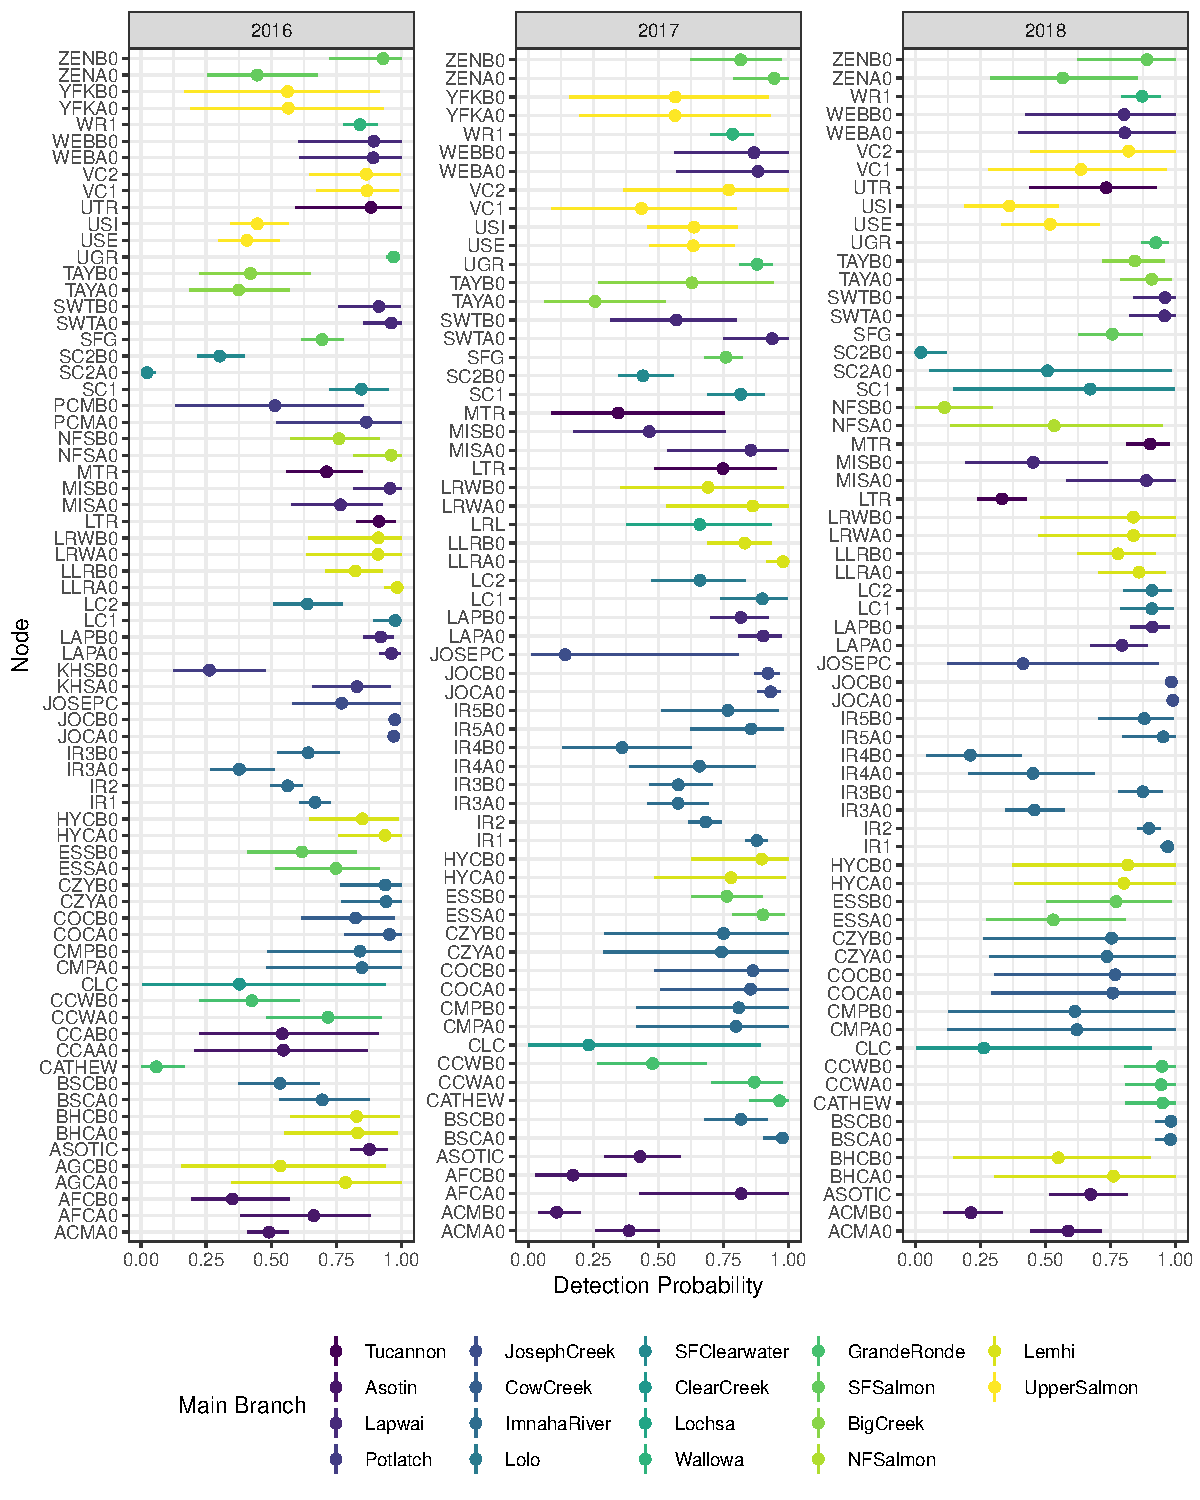
\includegraphics{'/Figures/DetectProp.pdf'}
\caption{Detection Probabilities.}
\end{figure}


\end{document}
